\documentclass[12pt,a4paper]{scrartcl}
\usepackage[utf8]{inputenc}
\usepackage[english,russian]{babel}
\usepackage{amssymb,amsfonts}
\usepackage{amsmath,cite,enumerate}
\usepackage{float,indentfirst}
\usepackage{graphicx}
\usepackage{geometry} % Меняем поля страницы
\geometry{left=2cm}% левое поле
\geometry{right=1.5cm}% правое поле
\geometry{top=1cm}% верхнее поле
\geometry{bottom=2cm}% нижнее поле
\graphicspath{{images/}}

\begin{document}


\begin{titlepage}
  \begin{center}
    Санкт-Петербургский Политехнический Университет     Петра Великого \\
    
    Институт компьютерных наук и технологий \\
    
    Кафедра компьютерных систем и программных технологий
  \end{center}
  
  \vfill
  
  \begin{center}
  Лабораторная работа №7\\
  по теме\\
  "Помехоустойчивое кодирование"\\
\end{center}

\vfill

\newlength{\ML}
\settowidth{\ML}{«\underline{\hspace{0.7cm}}» \underline{\hspace{2cm}}}
\hfill\begin{minipage}{0.4\textwidth}
  Выполнил студент группы 33501/3\\
  \underline{\hspace{\ML}} Кисличенко Б.\,Д\\
\end{minipage}%

\bigskip

\settowidth{\ML}{«\underline{\hspace{0.7cm}}» \underline{\hspace{2cm}}}
\hfill\begin{minipage}{0.4\textwidth}
  Руководитель\\
  \underline{\hspace{\ML}} Богач Н.\,В\\
\end{minipage}%

\vfill
 
\begin{center}
  Санкт-Петербург\\
2018 
\end{center}

\end{titlepage}

\section{Цель}
\label{sec:goal}

Изучение методов помехоустойчивого кодирования и сравнение их свойств.\\

\section{Постановка задачи}
\label{sec:task}

1) Провести кодирование/декодирование сигнала, полученного с помощью функции randerr  кодом Хэмминга 2-мя способами; с помощью встроенных функций encode/decode, а также через создание проверочной и генераторной матриц и вычисление синдрома. Оценить корректирующую способность кода.

2) Выполнить кодирование/декодирование циклическим кодом, кодом БЧХ, кодом Рида-Соломона. Оценить корректирующую способность кода.

\section{Коды кодирования}
\label{sec:teoriya}

\subsection{Циклические коды}
\label{sec:cycle_codes}

\textbf{Циклические коды} - подкласс линейных кодов, обладающие следующим свойством: циклическая подстановка символов в кодированном блоке дает другое возможное кодовое слово того же кода. Для работы с циклическими кодами в пакете Communications есть две функции. С помощью функции cyclpoly можно получить порождающий полином циклического кода. Для этого предварительно нужно задать число символов в кодируемом и закодируемом блоках. С помощью функции cyclegen и полученного раннее полинома можно получить порождающую и проверочную матрицы для данного кода.

\subsection{Коды БЧХ}
\label{sec:bchh_codes}

\textbf{Коды БЧХ} (Боуза — Чоудхури — Хоквингема) - являются подклассом циклических юлочных кодов. Для работы с ними есть функции bchenco (кодирование) и bcddeco (декодирование). Функция bchpoly позволяет расчитывать и считывать параметры или порождающий полином для двоичных кодов БЧХ.

\subsection{Коды Хэмминга}
\label{sec:hamming_codes}

\textbf{Коды Хэмминга} - подкласс циклических блочных кодов. Порождающий полином для кода Хэмминга - примитивен.  Длина кодированного блока равна 2m-1. Порождающая и проверочная матрицы для кодов Хэмминга генерируются функцией hammgen.

\subsection{Коды Рида-Соломона}
\label{sec:rid_solomon_g_codes}

\textbf{Коды Рида-Соломона} - подкласс циклических блочных кодов. Это единственные поддерживаемые пакетом Communications недвоичные коды. Для работы с этим кодом есть функции rsenco (кодирование) и rsdeco (декодирование). Функции rsencof и rsdencof осуществляют кодирование и декодирование текстового файла. Функция rspoly генерирует порождающие полиномы для кодов Рида-Соломона.

\clearpage
\newpage
\section{Ход работы}
\label{sec:work}

\subsection{Кодирование/декодирование кодом Хэмминга}
\label{sec:hamming}

%Рисунок 1
\begin{figure}[h!]
\center{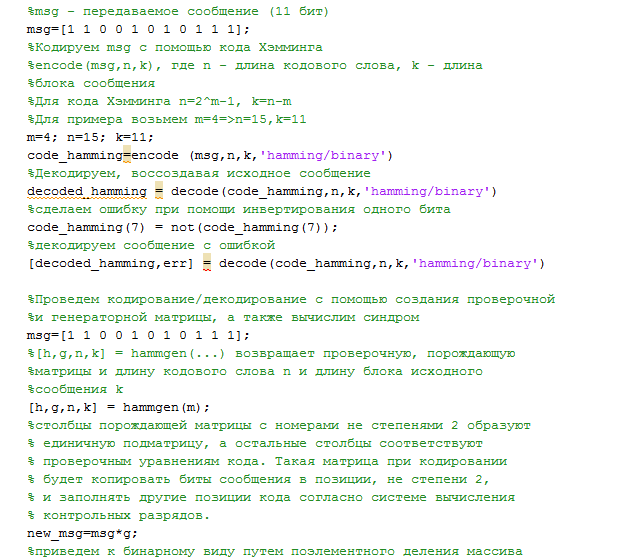
\includegraphics[width=0.9\linewidth]{hamming_code_1}}
\caption{Код Matlab (код Хэмминга) часть 1}
\end{figure}


\clearpage
\newpage

%Рисунок 2
\begin{figure}[h!]
\center{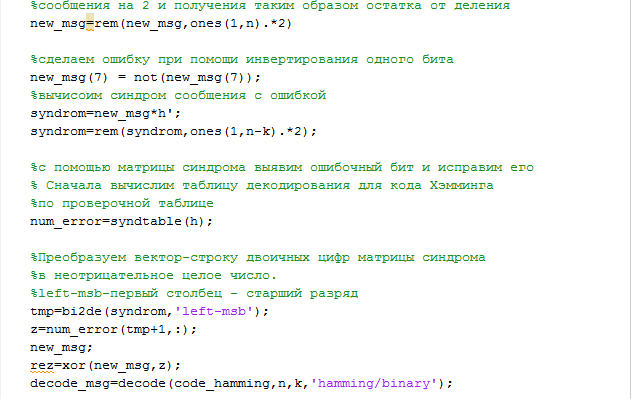
\includegraphics[width=0.9\linewidth]{hamming_code2}}
\caption{Код Matlab (код Хэмминга) часть 2}
\end{figure}

%Рисунок 3
\begin{figure}[h!]
\center{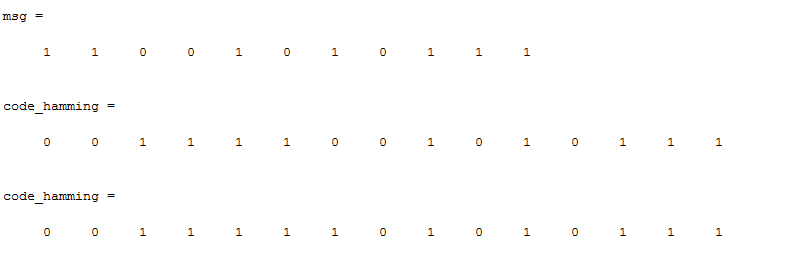
\includegraphics[width=0.9\linewidth]{hamming1}}
\caption{Сообщение, закодированное сообщение и закодированное сообщение с ошибкой в 7м разряде}
\end{figure}

%Рисунок 4
\begin{figure}[h!]
\center{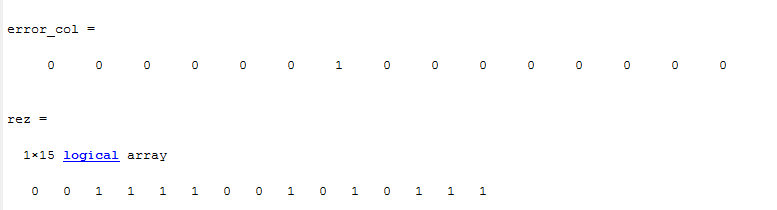
\includegraphics[width=0.9\linewidth]{hamming2}}
\caption{Номер разряда, в котором ошибка и исправленный результат}
\end{figure}

\clearpage
\newpage

\subsection{Кодирование/декодирование циклическим кодом}
\label{sec:cycle_code}

%Рисунок 5
\begin{figure}[h!]
\center{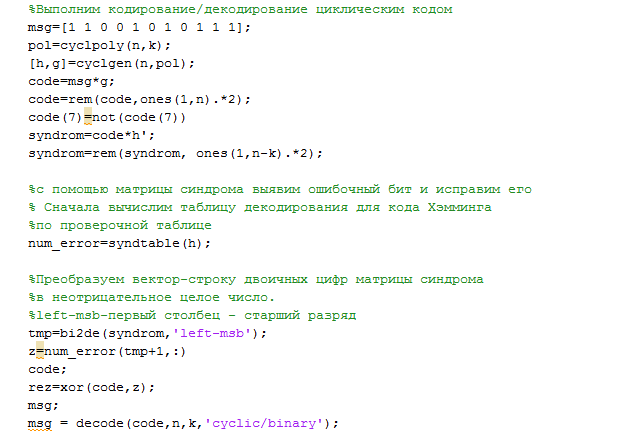
\includegraphics[width=0.9\linewidth]{cycle_code}}
\caption{Код Matlab (Циклический код)}
\end{figure}

%Рисунок 6
\begin{figure}[h!]
\center{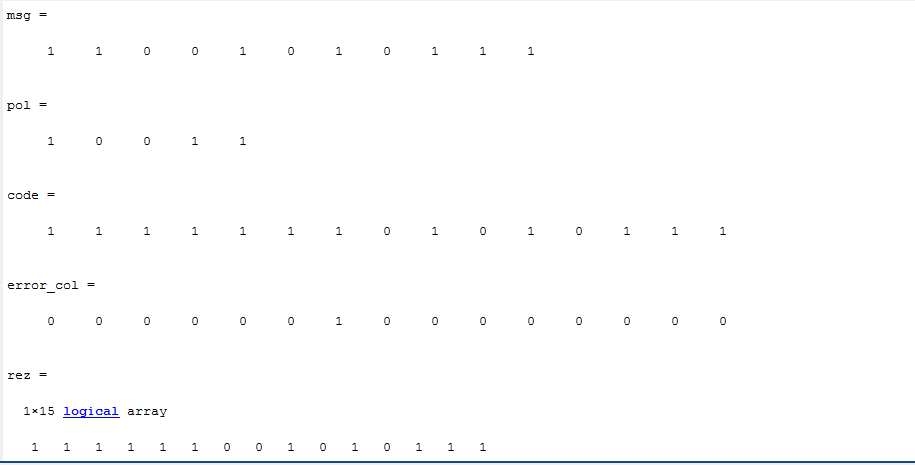
\includegraphics[width=0.9\linewidth]{cycle}}
\caption{Сообщение, полнином, сообщение в циклическом коде, номер разряда с ошибкой, исправленное закодированное сообщение}
\end{figure}

\clearpage
\newpage

\subsection{Кодирование/декодирование кодом БЧХ}
\label{sec:bchh}

%Рисунок 7
\begin{figure}[h!]
\center{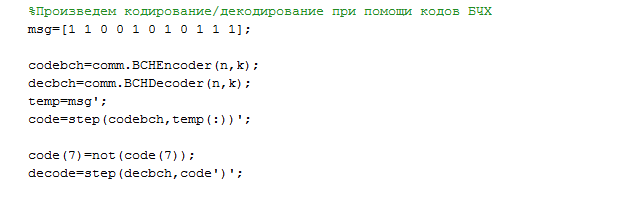
\includegraphics[width=0.9\linewidth]{bchh_code}}
\caption{Код Matlab (код БЧХ)}
\end{figure}

%Рисунок 8
\begin{figure}[h!]
\center{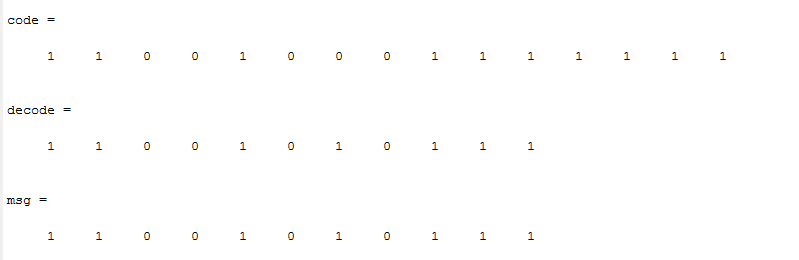
\includegraphics[width=0.9\linewidth]{bchh}}
\caption{сообщение в коде БЧХ, с ошибкой, декодированное сообщение}
\end{figure}

\clearpage
\newpage

\subsection{Кодирование/декодирование кодом Рида-Соломона}
\label{sec:bchh}

%Рисунок 9
\begin{figure}[h!]
\center{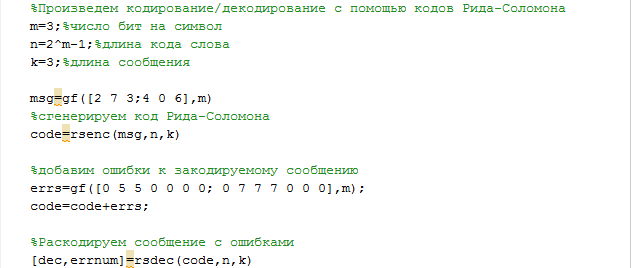
\includegraphics[width=0.9\linewidth]{rs_code}}
\caption{Код Matlab (код Рида-Соломона)}
\end{figure}

%Рисунок 10
\begin{figure}[h!]
\center{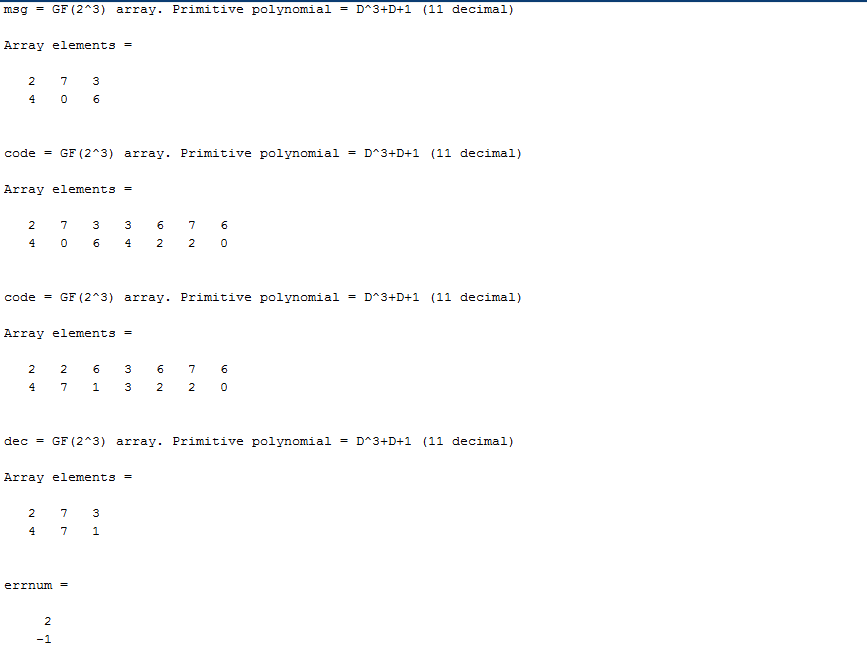
\includegraphics[width=0.9\linewidth]{rs}}
\caption{Передаваемое сообщение, сообщение в коде Рида-Соломона, с ошибкой, декодирование, кол-во ошибок}
\end{figure}

\clearpage
\newpage

\section{Вывод}
\label{sec:afterWork}
в ходе данной лабораторной работы были изучены методы помехоустойчивого кодирования и были сравнены их свойства. Исправляющая способность кодов Хэмминга, БЧХ, циклического кода равна 1. А исправляющая способность Рида-Соломона равна 2. Код Хэмминга используется в некоторых прикладных программах в области хранения данных. Коды Рида — Соломона имеют очень широкую область применения благодаря их способности находить и исправлять многократные пакеты ошибок. 

\end{document}